\documentclass[letterpaper, 10 pt, journal, twoside]{IEEEtran}
% \input{archive/main.config.tex}
\usepackage[maxnames=6,firstinits=true,doi=false,url=true,isbn=false]{biblatex}
% \addbibresource{IROS.bib}
\addbibresource{cav_tg.bib}
\usepackage{array}
\usepackage{graphicx}
\usepackage{amsmath}
\usepackage{amssymb}
\usepackage{color}
\usepackage{threeparttable}
\usepackage{balance} %balance columns
\hyphenation{op-tical net-works semi-conduc-tor}
\usepackage{enumitem}
\usepackage{hyperref} % Add  [ocgcolorlinks,pdfusetitle] before hyperref for colored links
% \usepackage{subfig}
\usepackage{subcaption}
\usepackage{dblfloatfix}
\usepackage{booktabs}
\usepackage{authblk}
\newcommand{\TODO}[1]{{\color{red}\textbf{TODO: #1}}}
% \pagenumbering{gobble} %suppresses page numbers
\usepackage{balance} %balance columns
% \usepackage{todonotes}
\usepackage[disable]{todonotes}
\usepackage{siunitx}
% \usepackage{draftwatermark}

%-------------------------------------------------------------------------------

\begin{document}

% ***************************************************
%  TITLE
% ***************************************************
\title{Test Generation Methods for Verification of Autonomous Systems}

\author{Kerstin Eder, Abanoub Ghobrial, Greg Chance, Severin Lemaignan, Tony Pipe  
\thanks{{\footnotesize
Manuscript  
received ...;
revised ...;  
accepted.... 
Date of publication ...;
date of current version ....

This research has in part been funded by the ROBOPILOT, CAPRI and CAVFOURTH projects. Both projects are part-funded by the Centre for Connected and Autonomous Vehicles (CCAV), delivered in partnership with Innovate UK under grant numbers 103703 (CAPRI) 103288 (ROBOPILOT) and 000000 (CAVFOURTH), respectively.
The Associate Editor for this paper was ....(\textit{Corresponding author: ....})

A.Ghobrial (e-mail: abanoub.ghobrial@bristol.ac.uk), 
G.Chance (e-mail: greg.chance@bristol.ac.uk), 
K.McAreavey (e-mail: kevin.mcareavey@bristol.ac.uk), 
and 
K.Eder (e-mail: kerstin.eder@bristol.ac.uk) 
are with the Trustworthy Systems Lab, Department of Computer Science, University of Bristol, Merchant Ventures Building, Woodland Road,  Bristol, BS8 1UQ, United Kingdom. 

S.Lemaignan (e-mail: severin.lemaignan@brl.ac.uk)
and
T.Pipe (e-mail: tony.pipe@brl.ac.uk), 
are with the Bristol Robotics Lab, T Block, University of the West of England,Frenchay, Coldharbour Ln, Bristol, BS34 8QZ, United Kingdom. 

Digital Object Identifier ....
}}}
\affil{Trustworthy Systems Laboratory, University of Bristol, Bristol, UK}
\affil{University of West of England, Bristol, UK}
\affil{Bristol Robotics Laboratory, Bristol, UK}

\markboth{IEEE TRANSACTIONS ON INTELLIGENT TRANSPORTATION SYSTEMS VOL. ..., NO. ..., date...}{Ghobrial \MakeLowercase{\textit{et al.}}: On Determinism of Game Engines used for Simulation-based Autonomous Vehicle Verification}

\maketitle
%
\begin{abstract}
\noindent 
Test generation...
        
\end{abstract}

\begin{IEEEkeywords}
Verification, Test Generation, Autonomous Vehicles, Simulation, Testing
\end{IEEEkeywords}
\IEEEpeerreviewmaketitle

% ***************************************************
%  INTRODUCTION
% ***************************************************
\section{Introduction} \label{s:introduction}

\IEEEPARstart{S}{}imulation-based verification...

\begin{figure}[!b]
    \centering
    \begin{subfigure}{.48\textwidth}
        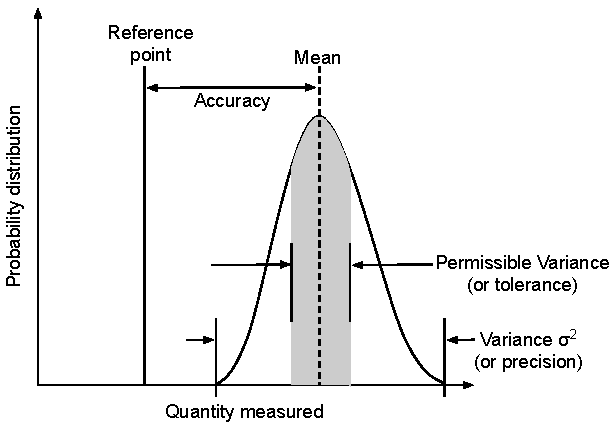
\includegraphics[width=1\textwidth]{Figures/Variance_predicition_tolerance_definition_diagram_a.pdf}
        \caption{Non-deterministic}
        \label{variance_description_a}
    \end{subfigure}
\end{figure}


% ***************************************************
%  INTRODUCTION - A Good Test Case
% ***************************************************

\subsection{A Good Test Case} \label{s:A Good Test Case}

What is considered a good test for an autonomous system? Are some methods better suited than others and will this depend on the application or context?

The following criteria for a ’good’ test case, which are inspired by [M. Fewster and D. Graham, Software test automation. Addison-Wesley Reading, 1999]: effectiveness in detecting failures, efficiency in minimising the number if tests required to achieve verification goals, economy in terms of resource usage and also robustness towards changes. 

In addition to this list our own thoughts on good tests are around: effectively generating coverage, maximising the entropy between test cases (similarity measure), have test cases that relate to national or international standards appropriate for the autonomous system (if available), be automated or have the ability to integrate within a testbench or testing pipeline with limited overhead, and have a high bug discovery rate.


% ***************************************************
%  Case Study
% ***************************************************
\section{Case Study}\label{s:Case Study}

How do we demonstrate if a method generates a `good' test case based on the requirements above? Can we also demonstrate the maturity of each method? Which methods can we rigorously and quantitatively assess?

Firstly which methods can we consider:
\newline - A random technique is good as it provides a baseline to reference other methods against.
\newline - Static test case (using GUI builder)
\newline - Dynamic test case (using game)
\newline - Algorithmic or agent based approach (Could we get this agent to adapt to the user's driving?)


% ***************************************************
%  Case Study - Data Gathering
% ***************************************************
\section{Data Gathering}\label{s:Data Gathering}


Participants are presented with 5 different driving objectives over 50 scenarios. In each scenario the user will have to achieve one of the 5 objectives but with a different test method each time. Therefore we use each method 10 times against the 5 objectives.

Participants control a vehicle in the simulation and aim to replicate the actions of an autonomous driving system. The list of 50 scenarios are presented randomly to minimise user learning. The objective is presented to the user at the start of each scenario. The actions of the actors within the environment are controlled by one of the 5 methods. Simulation logs are recorded noting the scenario number and the method used.


% ***************************************************
%  Case Study - Data Analysis
% ***************************************************
\section{Data Analysis}\label{s:Data Analysis}

Simulation logs are analysed against the criteria of a `good' test case.


% ***************************************************
%  Case Study - Results
% ***************************************************
\section{Results}\label{s:Results}

The results are summarised in Table 1.





% ***************************************************
%  CONCLUSION
% ***************************************************
\section{Conclusions \& Future Work}\label{s:conclusion}



% ***************************************************
%  FUNDING, REFS
% ***************************************************
% \section*{Acknowledgements}
% This research has in part been funded by the ROBOPILOT and CAPRI projects. Both
% projects are part-funded by the Centre for Connected and Autonomous
% Vehicles (CCAV), delivered in partnership with Innovate UK under grant numbers
% 103703 (CAPRI) and 103288 (ROBOPILOT), respectively.
\printbibliography

\end{document}
